% Least squares line y = 1/6 + x/2 through (0,0), (1,1), (2,1); residuals in red.
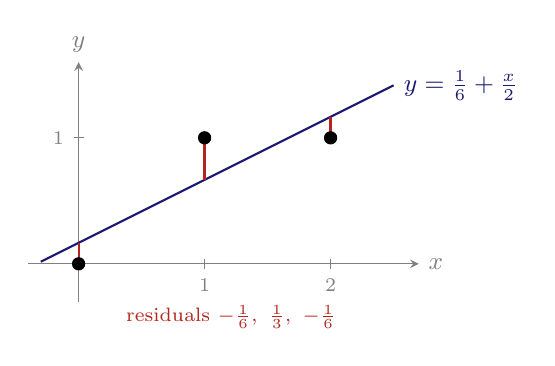
\begin{tikzpicture}[scale=1.6,>=stealth]
\draw[->,black!50] (-0.4,0) -- (2.7,0) node[right,font=\small] {$x$};
\draw[->,black!50] (0,-0.3) -- (0,1.6) node[above,font=\small] {$y$};
\draw[thick,MidnightBlue] (-0.3,0.0167) -- (2.5,1.4167) node[right,font=\small] {$y=\frac16+\frac x2$};
\draw[BrickRed,thick] (0,0) -- (0,0.1667);
\fill (0,0) circle (1.5pt);
\draw[BrickRed,thick] (1,1) -- (1,0.6667);
\fill (1,1) circle (1.5pt);
\draw[BrickRed,thick] (2,1) -- (2,1.1667);
\fill (2,1) circle (1.5pt);
\draw[black!50] (1,0.04) -- (1,-0.04) node[below,font=\scriptsize] {$1$};
\draw[black!50] (2,0.04) -- (2,-0.04) node[below,font=\scriptsize] {$2$};
\draw[black!50] (0.04,1) -- (-0.04,1) node[left,font=\scriptsize] {$1$};
\node[BrickRed,font=\scriptsize,anchor=west] at (0.3,-0.42) {residuals $-\frac16,\ \frac13,\ -\frac16$};
\end{tikzpicture}
